%%%%%%%%%%%%%%%%%%%%%%%%%%%%%%%%%%%%%%%%%
% Formal Book Title Page
% LaTeX Template
% Version 2.0 (23/7/17)
%
% This template was downloaded from:
% http://www.LaTeXTemplates.com
%
% Original author:
% Peter Wilson (herries.press@earthlink.net) with modifications by:
% Vel (vel@latextemplates.com)
%
% License:
% CC BY-NC-SA 3.0 (http://creativecommons.org/licenses/by-nc-sa/3.0/)
% 
% This template can be used in one of two ways:
%
% 1) Content can be added at the end of this file just before the \end{document}
% to use this title page as the starting point for your document.
%
% 2) Alternatively, if you already have a document which you wish to add this
% title page to, copy everything between the \begin{document} and
% \end{document} and paste it where you would like the title page in your
% document. You will then need to insert the packages and document 
% configurations into your document carefully making sure you are not loading
% the same package twice and that there are no clashes.
%
%%%%%%%%%%%%%%%%%%%%%%%%%%%%%%%%%%%%%%%%%

%----------------------------------------------------------------------------------------
%	PACKAGES AND OTHER DOCUMENT CONFIGURATIONS
%----------------------------------------------------------------------------------------

\documentclass[a4paper, 11pt, oneside]{book} % A4 paper size, default 11pt font size and oneside for equal margins


\usepackage{listings}
\usepackage{color}

\definecolor{dkgreen}{rgb}{0,0.6,0}
\definecolor{gray}{rgb}{0.5,0.5,0.5}
\definecolor{mauve}{rgb}{0.58,0,0.82}

\lstset{frame=tb,
  language=Java,
  aboveskip=3mm,
  belowskip=3mm,
  showstringspaces=false,
  columns=flexible,
  basicstyle={\small\ttfamily},
  numbers=none,
  numberstyle=\tiny\color{gray},
  keywordstyle=\color{blue},
  commentstyle=\color{dkgreen},
  stringstyle=\color{mauve},
  breaklines=true,
  breakatwhitespace=true,
  tabsize=3
}

\usepackage{url}
\usepackage{amsmath,hyperref}
\usepackage{graphicx}
\usepackage{float}
\usepackage[utf8]{inputenc} % Required for inputting international characters
\usepackage[T1]{fontenc} % Output font encoding for international characters
\usepackage{fouriernc} % Use the New Century Schoolbook font
\renewcommand\bibname{\Large\scshape References}
%----------------------------------------------------------------------------------------
%	TITLE PAGE
%----------------------------------------------------------------------------------------

\begin{document} 

\begin{titlepage} % Suppresses headers and footers on the title page

	\centering % Centre everything on the title page
	
	\scshape % Use small caps for all text on the title page
	
	\vspace*{\baselineskip} % White space at the top of the page
	
	%------------------------------------------------
	%	Title
	%------------------------------------------------
	
	\rule{\textwidth}{1.6pt}\vspace*{-\baselineskip}\vspace*{2pt} % Thick horizontal rule
	\rule{\textwidth}{0.4pt} % Thin horizontal rule
	
	\vspace{0.75\baselineskip} % Whitespace above the title
	
	{\LARGE Implementation of Bittorrent-like algorithem Using UDP
with Reliability and Congestion Control\\} % Title
	
	\vspace{0.75\baselineskip} % Whitespace below the title
	
	\rule{\textwidth}{0.4pt}\vspace*{-\baselineskip}\vspace{3.2pt} % Thin horizontal rule
	\rule{\textwidth}{1.6pt} % Thick horizontal rule
	
	\vspace{2\baselineskip} % Whitespace after the title block
	
	%------------------------------------------------
	%	Subtitle
	%------------------------------------------------
	
	CS:6250 Computer Networks - Project Final Report
	
	\vspace*{3\baselineskip} % Whitespace under the subtitle
	
	%------------------------------------------------
	%	Editor(s)
	%------------------------------------------------
	
Team 11: Mansour Alharthi, Jiahao Cui, Peicheng Hua, Hao Fu, Nan Zhang	
	
		
	\vspace{2\baselineskip} % Whitespace below the editor list
	
	For: Dr. Mostafa Ammar

	
	\vspace{1.5\baselineskip} % Whitespace below the editor list
	
	\textit{Georgia Institute of Technology} 



\end{titlepage}
\section*{\scshape Introduction}
BitTorrent, one of the most widespread file sharing P2P applications, has recently been
updated to eliminate use of TCP by introducing an application-level congestion control
protocol \cite{Arvid}. This new protocol aims to efficiently use the available link capacity while
avoiding interference with other user traffic (e.g., Web, VoIP, and gaming) sharing the
same access link. In this project, we aim to simulate this protocol in a virtual
network environment. Because of the high complexity of Bittorrent, a full Bittorrent protocol implementation is not feasible; instead, we will implement a Bittorrent-like
protocol to demonstrate its functionality. 

\section*{\scshape Design}
\begin{figure}[H]
\centering
   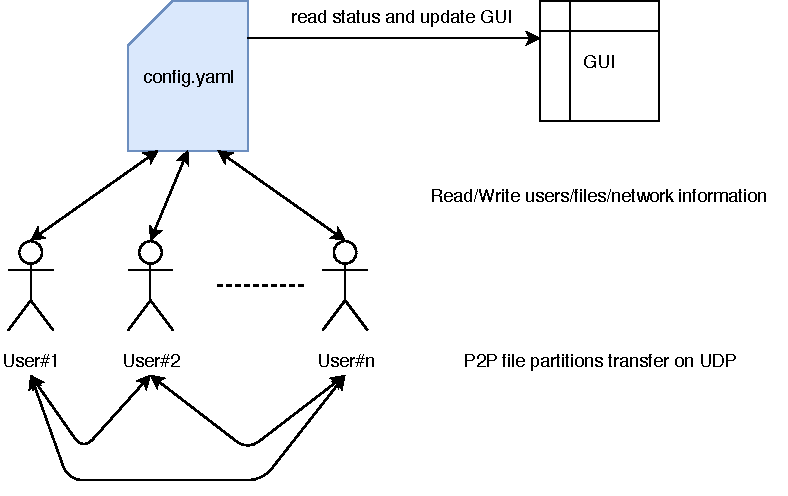
\includegraphics[width=1\linewidth]{design}
   \caption{The design of Bittorrent-like protocol}
   	\label{fig:design}
\end{figure}
Our protocol design objectives are as follows: 
\begin{enumerate}
\item \textbf{Fairness among users.} We ensure fairness by dividing available bandwidth among users by equal shares. 
\item \textbf{Fairness to network traffic.} We ensure fairness to network traffic by detecting congestion control and sensing available network bandwidth. 
\item \textbf{Link utilization.} Our design satisfy link utilization requirements by dividing available bandwidth only to active users. 
\item \textbf{Transparent network status.} Our design includes an easy-to-read Graphical User Interface; allowing the user to monitor the network status. 
\end{enumerate}

The design of our protocol is shown in \autoref{fig:design}. When a user wishes to download a file, it will first query a central \texttt{config.yaml} file that contains information about available users, existing files in the peers network, and the network status. Then, the user will initiate a file request from peers that own the requested file; keeping in mind the available bandwidth allocated to him in \texttt{config.yaml}. The new user will also update the \texttt{config.yaml} to add his own information, and update the network status information.  A Graphical User Interface is updated periodically to reflect changes made in the \texttt{config.yaml}. An example of \texttt{config.yaml} is shown in \autoref{lis:config}.

\begin{lstlisting}[caption={Example \texttt{config.yaml} file},captionpos=b, label={lis:config}]

available: 138
file_info:
  filename1:
    file_size: 60
    hostsWithFile:
    - {ip: 127.0.0.1, port: 8080}
    - {ip: 127.0.0.2, port: 8081}
    - {ip: 127.0.0.3, port: 8082}
  filename2:
    file_size: 100
    hostsWithFile:
    - {ip: 127.0.0.1, port: 8080}
    - {ip: 127.0.0.2, port: 8081}
    - {ip: 127.0.0.3, port: 8082}
lock: false
network_info:
  activeUsers:
  - {ip: 127.0.0.1, port: 8080}
  - {ip: 127.0.0.2, port: 8081}
  - {ip: 127.0.0.3, port: 8082}
  available: 138
  bandwidth: 100
  threshold: 80
  total_time: []
total_time: [4.031458854675293, 4.0014543533325195, 3.9738223552703857, 3.9723050594329834,
  3.9719390869140625, 3.972656726837158, 3.9447362422943115, 3.9431591033935547, 3.9433462619781494,
  3.9440770149230957, 3.9153740406036377]
\end{lstlisting}


\section*{\scshape Implementation}
\subsection*{\scshape Part 1}


\subsection*{\scshape Part 2}


\subsection*{\scshape Part n}




\subsection*{\scshape Graphical User Interface}
The Graphical User Interface should reflect current peer network status based on information read from \texttt{config.yaml}. Given the frequency the configuration file changes with, the GUI content will expire every second, and a content update will occur. \autoref{fig:gui} shows our GUI design. We implemented the GUI code using \texttt{Python}, utilizing the \texttt{PyQt4} library.
\begin{figure}[H]
\centering
   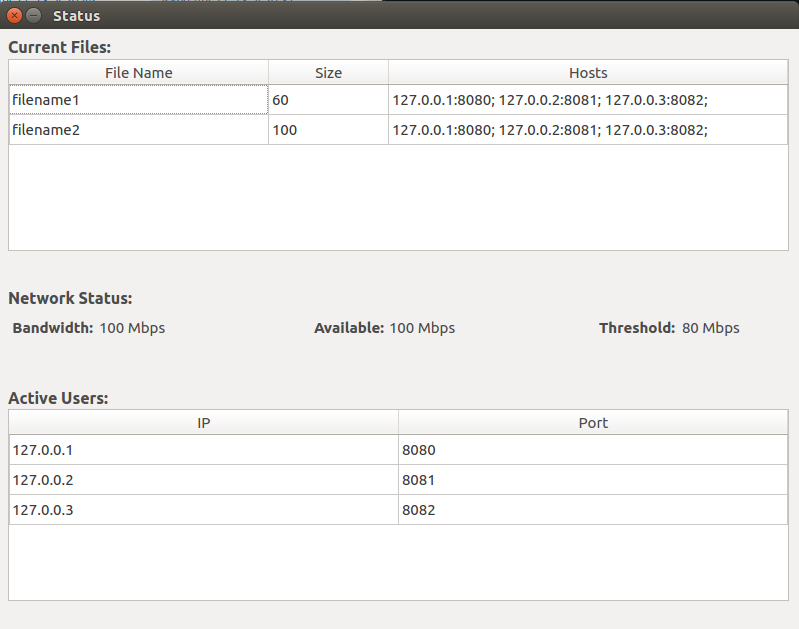
\includegraphics[width=1\linewidth]{gui}
   \caption{A GUI showing current peer network status}
   	\label{fig:gui}
\end{figure}


\section*{\scshape Evaluation}
\subsection*{\scshape Concurrent Download}
Show the speed of concurrent download in our implementation. Maybe simulate packet loss to test error detection?

\subsection*{\scshape Comparison with TCP}
Compare our results with concurrent download using TCP. Simulate packet loss. 




\section*{\scshape Discussions}
\paragraph{Equal Sharing.} Our design divides the available bandwidth among active users in equal shares. Although this ensures fairness among users, it also may lead to inefficient link utilization if the user bandwidth demand is less than equal share. 

\paragraph{Other points to discuss? }

\section*{\scshape Conclusion}
We designed and implemented a peer-to-peer file transfer protocol that ensures fairness to users and network traffic. We tested our implementation against concurrent TCP connection downloads. Our results show that our implementation provide XXXX increase in download speed over concurrent TCP connections download. 

\begin{thebibliography}{999}

\bibitem{Arvid}
  Arvid Norberg,
  \emph{uTorrent transport protocol}.
  \url{http://www.bittorrent.org/beps/bep_0029.html}

\end{thebibliography}
\end{document}
